\subsubsection*{Precipitate dissolution modeling}

This is an property estimation problem with one input variable, one output variable and one independent parameter. 
The mathematical model here is expressed as an algebraic equation. 

The objective is to model the dissolution rate of hardening precipitates in aluminium alloys. 
The effective activation energy is also in unison determined as that providing the best results. 
Aluminium alloys 2014-T6 and 7449-T79 are considered. 
Figure \ref{VickersTesterFigure} shows a Vickers hardness tester (picture from Wikipedia). 

\begin{figure}[h!]
\begin{center}
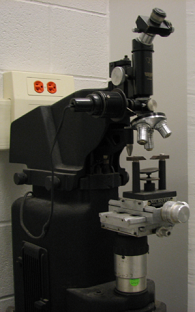
\includegraphics[width=0.5\textwidth]{inverse_problems/vickers_tester}
\caption{Vickers hardness tester.}\label{VickersTesterFigure}
\end{center}
\end{figure}

Assuming that the nucleation of precipitates is
negligible compared to the dissolution of precipitates, the
following linear relationship between the Vickers hardness and the
volumetric fraction of precipitates can be established
\cite{Myrh1991b}.

The Vickers hardness equation is extremely useful since the
hardness is much easier to measure than the relative volume
fraction of precipitates.

The dissolution modeling process is to estimate an activation
energy providing minimum dispersion for the experimental data
while a function providing minimum error.
Mathematically, this can be formulated as a variational problem
including independent parameters.

Experimental tests have been performed in order to get the
isothermal time evolution of Vickers hardness at different
temperatures and for various aluminium alloys. In particular, two
materials have been used for the isothermal heat treatments, 2014-T6
and 7449-T79 aluminium alloys.

The Vickers hardness data for aluminium alloy 2014-T6 is taken from
\cite{Shercliff2005}, while that for aluminium alloy 7449-T79 is
obtained from an independent test performed within the DEEPWELD
Specific Targeted Research Project (STREP) co-funded by the 6th
Framework Programme of the European Community (AST4-CT-2005-516134).

Figures \ref{VickersHardnessTest2014-T6} and
\ref{VickersHardnessTest7449-T79} depict these Vickers hardness test
for aluminium alloys 2014-T6 and AA7449-T6, respectively. Note that,
in both figures the Vickers hardness decreases with the time, due to
dissolution of hardness precipitates.

\begin{figure}[h!]
\begin{center}
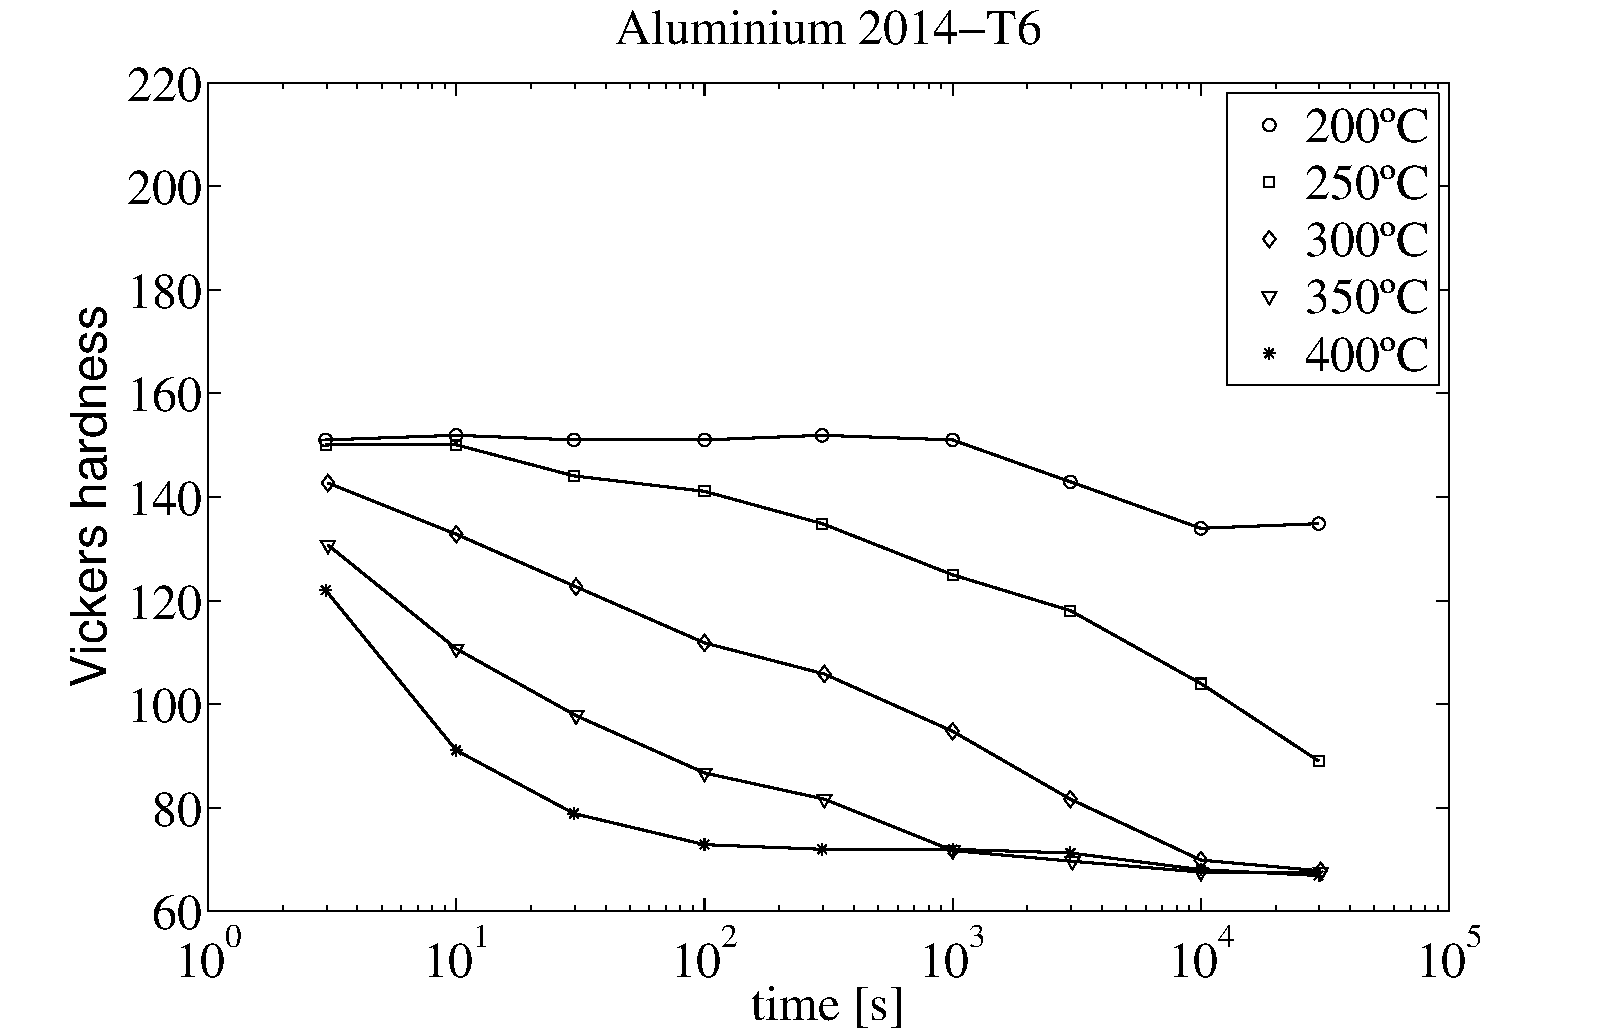
\includegraphics[width=0.9\textwidth]{inverse_problems/vickers_hardness_test_2014-T6}
\caption{Vickers hardness test for aluminium alloy
2014-T6.}\label{VickersHardnessTest2014-T6}
\end{center}
\end{figure}

\begin{figure}[h!]
\begin{center}
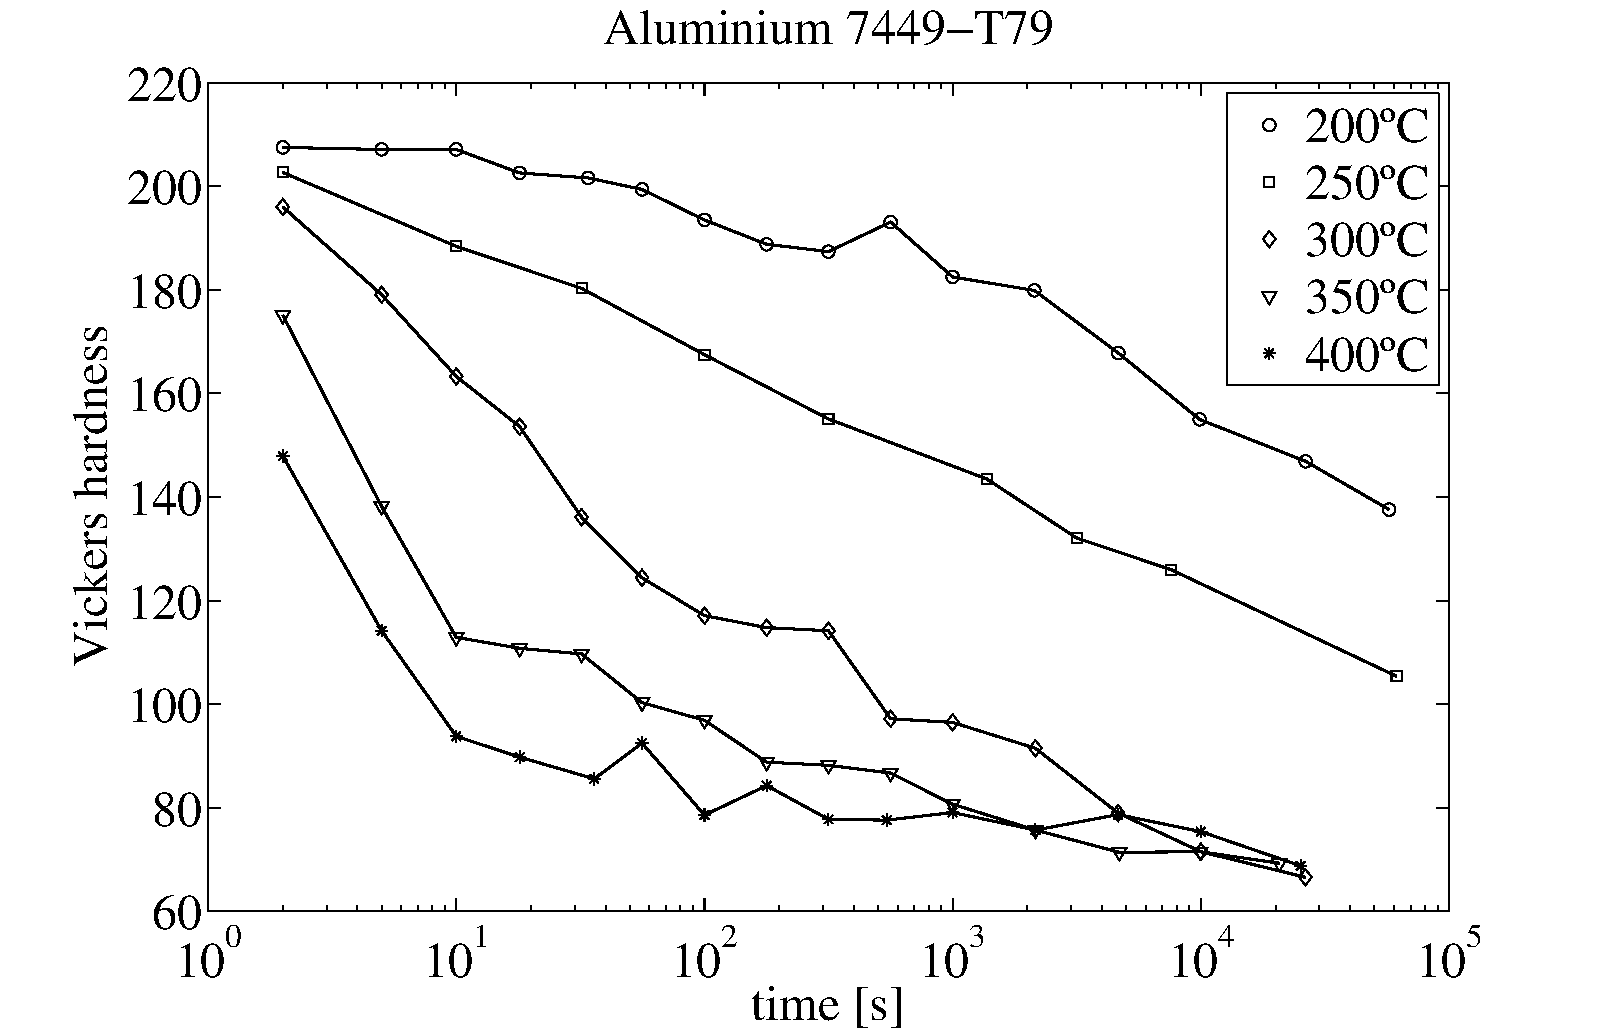
\includegraphics[width=0.9\textwidth]{inverse_problems/vickers_hardness_test_7449-T79}
\caption{Vickers hardness test for aluminium alloy
7449-T79.}\label{VickersHardnessTest7449-T79}
\end{center}
\end{figure}
